\documentclass{article}
\usepackage{amsmath}
\usepackage{xcolor}
\usepackage{biblatex}
\usepackage{graphicx}
\usepackage{listings}
\lstset{
  basicstyle=\ttfamily,
  columns=fullflexible,
  breaklines=true,
  postbreak=\raisebox{0ex}[0ex][0ex]{\color{red}$\hookrightarrow$\space}
}
\usepackage{geometry}
 \geometry{
 a4paper,
 total={170mm,257mm},
 left=20mm,
 top=20mm,
 }

\begin{document}
\pagenumbering{gobble}
	\title{Project Cecropia}
	\author{Yilun "Allen" Chen}
  	\newpage
    \pagenumbering{arabic}
\begin{titlepage}
  \begin{center}
      \vspace*{8cm}

      \textbf{Project Cecropia}

      \vspace{0.5cm}
       Training Manual for the Integrated Server for the SlothBot 

      \vspace{1.5cm}

      \textbf{Yilun "Allen" Chen}

      \vfill


      Robotarium\\
      Georgia Institute of Technology\\
      United States\\
      June 30th, 2019

  \end{center}
\end{titlepage}

\tableofcontents
\newpage

\section{Overview}
\subsection{Abstract}
\paragraph{} Project Cecropia aims to provide real-life application for the SlothBot swarm. The SlothBots are fall-safe
wire-traversing robots developed in Robotarium at Georgia Tech. They will later be deployed to Atlanta Botanical Garden for enviornment monitoring
purposes. Project Cecropia offers a solution to allow the collection of the data trasmitted from the SlothBots, along with the capability to store
and visualize the data on a web page that it serves.
\paragraph{}This document aims to provide an overview of how the project works for future developers of the project. Details of how the project is structured, 
how it achieves different functionalities, how to deal with emergencies/bugs will be provided.
\paragraph{}
\paragraph{}
\begin{center}
  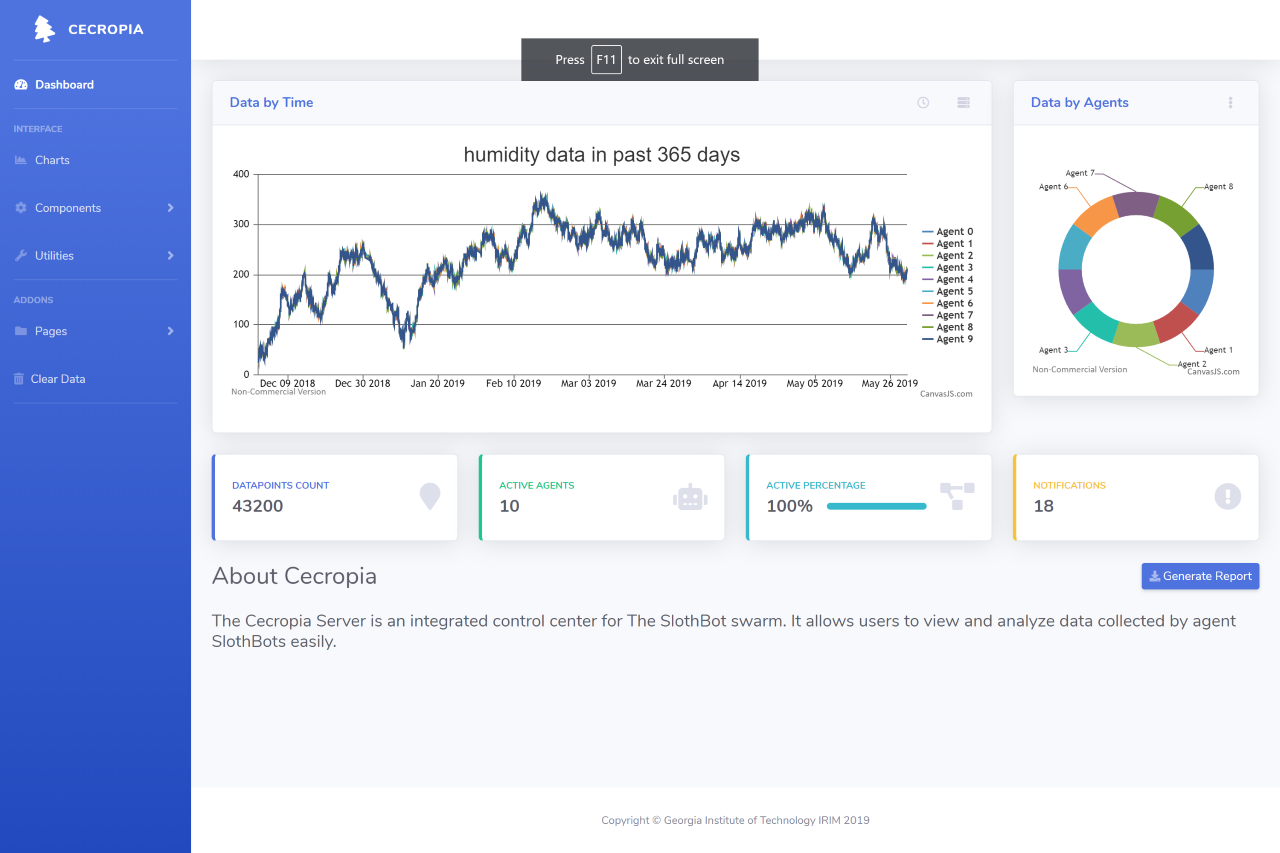
\includegraphics[scale=0.5]{sample}
  Figure 1. GUI screenshot of the Cecropia system.
\end{center}



\newpage
\subsection{Tech Stack}
Here is a general overview of how the project is structured. Main building blocks of the project and their rationales are provided, 
so that future developers of the project may use this as a reference.
\paragraph{Web Framework:} Express \& Node.js\\
Node.js as a web framework has high integrity when it comes to building web applications. Its package manager 
NPM offers a wide variety of packages, providing almost all functionalities desired. 
\paragraph{Database:} MongoDB\\
MongoDB uses JSON-like syntax as the form of its document. This feature/characteristic means that its documents
can be easily translated into a form that is easy for JavaScript to use.
\paragraph{User Interface:} JQuery \& Bootstrap\\
jQuery and Bootstrap offer a wide choice of templates that we can straight up use and build upon, while adding a lot of additional 
handy functionalities that can be used in overall development process.
\paragraph{Package Management:} NPM\\
Almost all JavaScript packages can be found on NPM. It is extremely easy to use and it also offers great mobility - When 
you try to move the server to another host, you can easily setup the needed environment.
\paragraph{Data Visualization:} CanvasJS (JavaScript Library)\\
Canvas JS is a licensed JavaScript library that allows you to create graphs with massive amount of data points. It has superb performance in 
handling mass data and is highly configurable.
\paragraph{Server/Data Visualization API: } DataParser (Customized JavaScript function)\\
A customized JavaScript class that takes in all the data points retrieved, sort them by timestamp and dates and outputs a CanvasJS-friendly
cluster of data to be put directly into the data-visualization process.
\paragraph{Testing Platform: } RDP.py (Customized Python Script)\\
A script to generate continuous mock data and send it over to the server. Depends on the pacakge 'request'.

\newpage
\section{Design Roadmap}
\subsection{Design Constraints}
\subsubsection{Power Consumption: } Due to the moving nature of the SlothBots, they will not be relying on stationary charging stations, but instead, their only source of power is 
the solar panels they carry with them. This means that we want to minimize the power consumption of the SlothBots so that they run longer before they take another 'power nap'.
\subsubsection{Mass Data Handling: } Because the number of robots deployed is unknown, and that we are collecting a huge amount of various kinds of data, we must ensure that the server
is capable of retrieving only the necessary data, and that it has the capability of properly handle these data.
\subsubsection{Connection-Failure-Safe: } In case that the server goes offline, the data already collected should be preserved. 
\subsubsection{Centralized Data Processing: } An entry point to all the data collected is required. This means that all the data collected by the agent robots must be re-collected by one 
machine and can therefore be processed.

\subsection{Current Solutions}
\subsubsection{Stationary Server} As of for now the server is deployed onto a stationary computer that runs continuously under a stable network with internet access.
This provides a resolution to seemingly conflicting design constraints by putting the load of performance-heavy works onto a device that has access to a steady source of power.
Agent Robots can now only be responsible for transferring the data, without wasting the power to process them.
\subsubsection{Integrated Database} The server will be interacting with an independent database that runs alongside it. This means that even if the server encounters an error, the database will still be preserved.
Also, because MongoDB is a NoSQL database, even if the server is injected with false/garbage data, the database will still be able to function properly.


\subsection{Expandabilities}
\subsubsection{Network Connection Check on the SlothBots When Sending Data} Currently the programs that run on the SlothBots are still work-in-process. Ideally they would automatically detect the quality of 
their internet connections and in case they are unable to send over the data, they would save the data in a cache, and once they regain proper connection, send all the data 
over to the server since the connection breaks down. The server is already capable of dealing with multiple entries per request and it is also capable of sorting the data points
by their time stamps.
\subsubsection{Database With Better Performance} MongoDB is not the best performance-wise and space-wise when it comes to massive data (More than hundreds of data entries, for example). If we were to deal with this 
amount of data entries, it is a good idea to switch over to SQL databases like MySQL. This, however, requires the developers to develop a query system to let the server and the database communicate properly.



\newpage
\section{Building Blocks}
This section aims to introduce the readers what each individual module in the project does, so that in case of errors, the developers can quickly 
locate the problem and solve it. Only the modules used in real deployment will be discussed.
\subsection{app.js}
\begin{itemize}
  \item Modules Management: It loads in all the required modules.
  \item Establish Connection: It setup express and starts to serve on desired IP.
  \item Database Connection: It attempts to connect to MongoDB via port 27017.
  \item It routes different request to different sites.
  \begin{itemize}
    \item /visitor: Dashboard of the system, where users can obtain data.
    \item /dataPost: Interface between robots and the system. Used to post data.
    \item /clearData: Used to clean up all data stored in the database. 
  \end{itemize}
\end{itemize}

\subsection{dashboard.html}
\begin{itemize}
  \item It is a html file that will first be processed on the server side (replace data place holder by real data) then sent over to the client's side to be rendered.
\end{itemize}

\subsection{dataParser.js}
\begin{itemize}
  \item It takes in all the data entries and put data points of individual agent into its own bucket.
  \item It sorts the data points by their timestamps.
  \item It generates strings to be replaced in dashboard.html file that is readable by CanvasJS.js to visualize.
\end{itemize}

\subsection{Miscellaneous}
\begin{itemize}
  \item canvasjs.min.js: Should be left untouched.
  \item All files under node\_modules: Dependencies for the project to function properly. Should be left untoucched.
  \item All files under vendor: GUI components of the project. Should be left untouched.
  \item sb-admin-2.min.css: CSS file for the dashboard. Should be left untouched.
\end{itemize}


\newpage
\section{Troubleshooting}
\subsection{Address Not Available}
\paragraph{} This corresponds to the following lines in app.js. Check if the your IP address aligns with the setting.
\begin{lstlisting}
  const hostname = '192.168.137.1';
  const app = express();
  const port = 80;  
\end{lstlisting}

\subsection{connect ECONNREFUSED}
\paragraph{} This means that your mongoDB is not set to connect on the right port. The default port is 27017.

\subsection{Data Visualization Failure}
\paragraph{} Many errors can lead to failure to visualize data. Try to use RDP.py (Random Data Poster) as a testing tool. If the server logs "new data received" in console then it means that 
the connection with the database is intact. If no data is received, check the connection with the database, or the internet connections of your devices.
\paragraph{} Assuming that your connection is intact: At this point, check if the data from RDP.py can be displayed, then check the formatting of your post requests. However if
it not being able to display RDP data, it means that dataParser is malfunctioning and a debugging session with DataParser.js is highly recommended.


\section{Data Formatting Examples}
\subsection{Post Requests}Post Requests of the agent robots should follow this format:
\begin{lstlisting}
  {"dataType":"temperature","timeStamp":2019011020,"dataValue":255,"signature":1}
\end{lstlisting}

\subsection{Document Entry in MongoDB} A document (or data entry) in MongoDB has the following format:
\begin{lstlisting}
  {"_id":"5cfe784f903ad52ee0cad536","dataType":"temperature",
   "timeStamp":2019011020,"dataValue":255,"signature":1}
\end{lstlisting}

\subsection{String Processed by DataParser} The data after being processed by DataParser.js should have the following format:
\begin{lstlisting}
  {
  "type":"line",
  "showInLegend":true,
  "legendText":"Agent 0",
  "xValueType":"dateTime",
  "dataPoints":[
    {"x":1558360800000,"y":86},
    {"x":1558368000000,"y":91},
    {"x":1558375200000,"y":97},
    {"x":1558382400000,"y":97},
    {"x":1558389600000,"y":99},
    {"x":1558396800000,"y":93},
    {"x":1558404000000,"y":92},
    {"x":1559253600000,"y":47}
    ]
  }
\end{lstlisting}


\end{document}